% ===========================================================
%  Лекция 14. Алгоритм Флойда. Алгоритм Джонсона
% ===========================================================

\chapter{Лекция 14. Алгоритм Флойда. Алгоритм Джонсона}

% ===========================================================
%  Алгоритм Флойда (подробный пример)
% ===========================================================

\begin{algo}{Алгоритм Флойда}{floyd}

$G(V, E)$~--- слабо связный ориентированный граф, $\sigma\colon E \to \mathbb{R}$.

Алгоритм аналогичен Флойду--Уоршеллу. На каждом шаге выделяем ведущую вершину (строку и столбец), проверяем все пересечения.

\textbf{Хранение пути:} для пары $(u, w)$ храним $P_{uw}$~--- первую путевую точку. Для прямого ребра $A \to B$~--- ничего хранить не надо. Остаток пути: $B \to \ldots \to L$.

Если $\mu(u,w) > \mu(u,v) + \mu(v,w)$, то $\mu(u,w) := \mu(u,v) + \mu(v,w)$, $P_{uw} := P_{uv}$ (или $v$, если $P_{uv}$ пуст).

\textbf{Пример} (рис.~p32-f-example-1): граф $A, B, C, D$.

Список рёбер с весами:
\begin{center}
\begin{tabular}{cc}
Ребро & Вес \\
\hline
$AB$ & 1 \\
$BC$ & 1 \\
$BD$ & 3 \\
$CA$ & $-2$ \\
$CD$ & 1 \\
$DA$ & 4 \\
\end{tabular}
\end{center}

\grfig[0.45]{figures/p32-f-example-1.pdf}{Алг. Флойда: $A,B,C,D$ ($AB{=}1$, $BC{=}1$, $BD{=}3$, $CA{=}-2$, $CD{=}1$, $DA{=}4$)}

Шаг~0 (инициализация):
\begin{center}
\begin{tabular}{c|cccc}
     & $A$      & $B$      & $C$      & $D$      \\
\hline
$A$  & 0        & 1        & $\infty$ & $\infty$ \\
$B$  & $\infty$ & 0        & 1        & 3        \\
$C$  & $-2$     & $\infty$ & 0        & 1        \\
$D$  & 4        & $\infty$ & $\infty$ & 0        \\
\end{tabular}
\end{center}

Шаг~1 (ведущая $A$): выделяем строку $A$ и столбец $A$. Обновления: $\mu(C,B)\colon \infty > (-2) + 1 = -1$; $\mu(D,B)\colon \infty > 4 + 1 = 5$.
\begin{center}
\begin{tabular}{c|cccc}
     & $A$      & $B$      & $C$      & $D$      \\
\hline
$A$  & 0        & 1        & $\infty$ & $\infty$ \\
$B$  & $\infty$ & 0        & 1        & 3        \\
$C$  & $-2$     & $-1, A$  & 0        & 1        \\
$D$  & 4        & $5, A$   & $\infty$ & 0        \\
\end{tabular}
\end{center}

Шаг~2 (ведущая $B$): обновления: $\mu(A,C)\colon \infty > 1 + 1 = 2$; $\mu(A,D)\colon \infty > 1 + 3 = 4$; $\mu(D,C)\colon \infty > 5 + 1 = 6$.
\begin{center}
\begin{tabular}{c|cccc}
     & $A$      & $B$      & $C$      & $D$      \\
\hline
$A$  & 0        & 1        & $2, B$   & $4, B$   \\
$B$  & $\infty$ & 0        & 1        & 3        \\
$C$  & $-2$     & $-1, A$  & 0        & 1        \\
$D$  & 4        & $5, A$   & $6, A$   & 0        \\
\end{tabular}
\end{center}

Шаг~3 (ведущая $C$): обновления: $\mu(A,D)\colon 4 > 2 + 1 = 3$; $\mu(B,A)\colon \infty > 1 + (-2) = -1$; $\mu(B,D)\colon 3 > 1 + 1 = 2$.
\begin{center}
\begin{tabular}{c|cccc}
     & $A$      & $B$      & $C$      & $D$      \\
\hline
$A$  & 0        & 1        & $2, B$   & $3, B$   \\
$B$  & $-1, C$  & 0        & 1        & $2, C$   \\
$C$  & $-2$     & $-1, A$  & 0        & 1        \\
$D$  & 4        & $5, A$   & $6, A$   & 0        \\
\end{tabular}
\end{center}

Шаг~4 (ведущая $D$): нет изменений (все пути через $D$ дороже найденных).
\begin{center}
\begin{tabular}{c|cccc}
     & $A$      & $B$      & $C$      & $D$      \\
\hline
$A$  & 0        & 1        & $2, B$   & $3, B$   \\
$B$  & $-1, C$  & 0        & 1        & $2, C$   \\
$C$  & $-2$     & $-1, A$  & 0        & 1        \\
$D$  & 4        & $5, A$   & $6, A$   & 0        \\
\end{tabular}
\end{center}

\medskip
\noindent\textbf{Работа алгоритма по шагам.} Ведущая вершина ---
оранжевая; найденные на текущем шаге кратчайшие обходы --- зелёные дуги
с новой длиной, найденные ранее --- светло-фиолетовые:

\begin{center}\begin{tabular}{ccc}
\shortstack{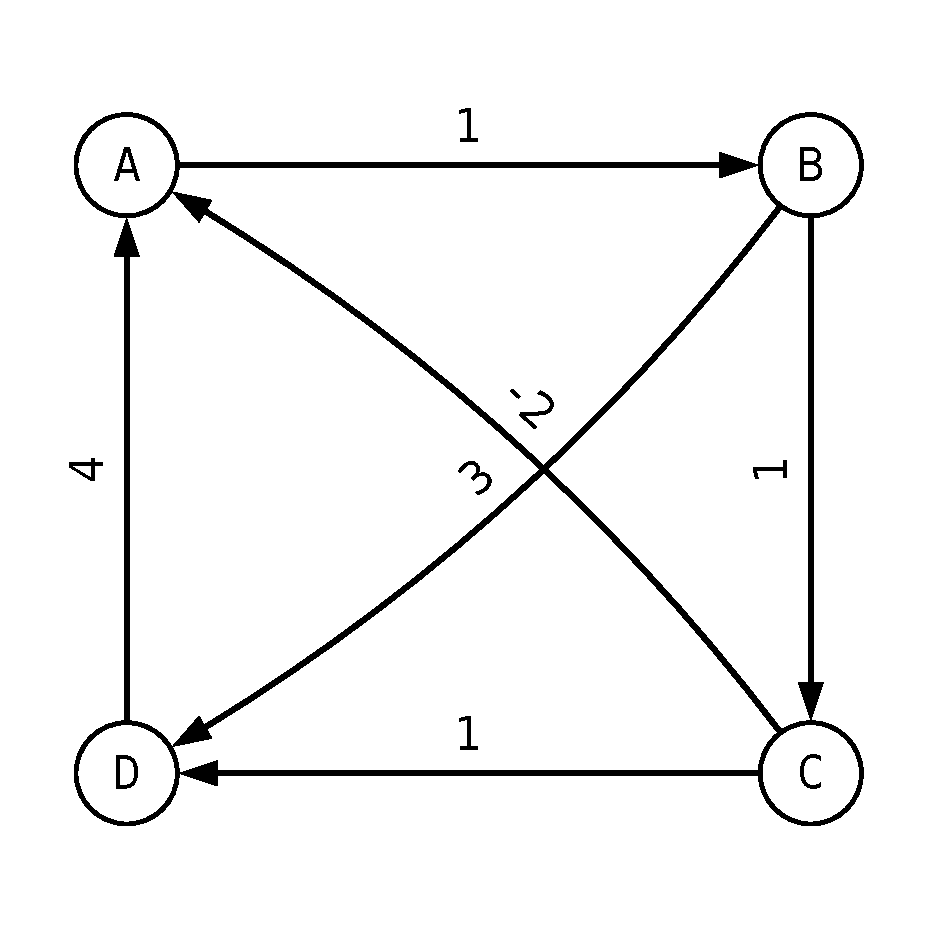
\includegraphics[width=0.30\textwidth]{python/lec14/floyd/floyd-0.pdf}\\[2pt]{\scriptsize Шаг 0. Исходный граф}} &
\shortstack{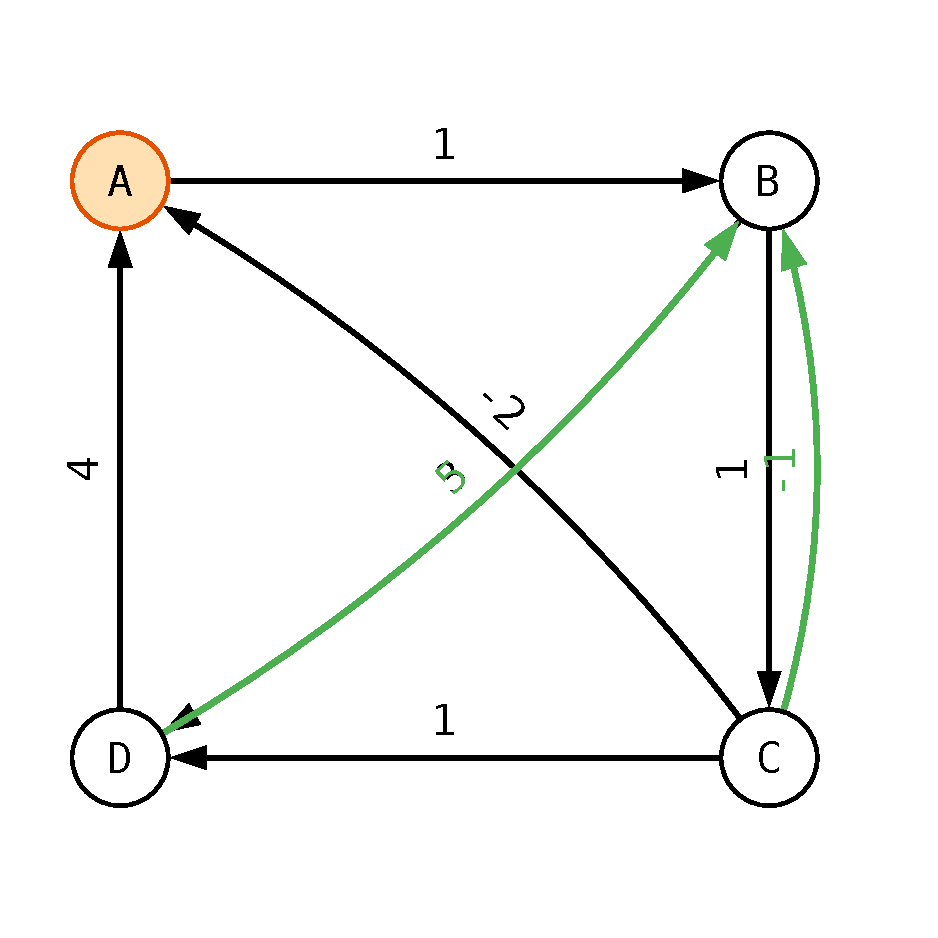
\includegraphics[width=0.30\textwidth]{python/lec14/floyd/floyd-1.pdf}\\[2pt]{\scriptsize Шаг 1. Через $A$: $CB{=}{-}1$, $DB{=}5$}} &
\shortstack{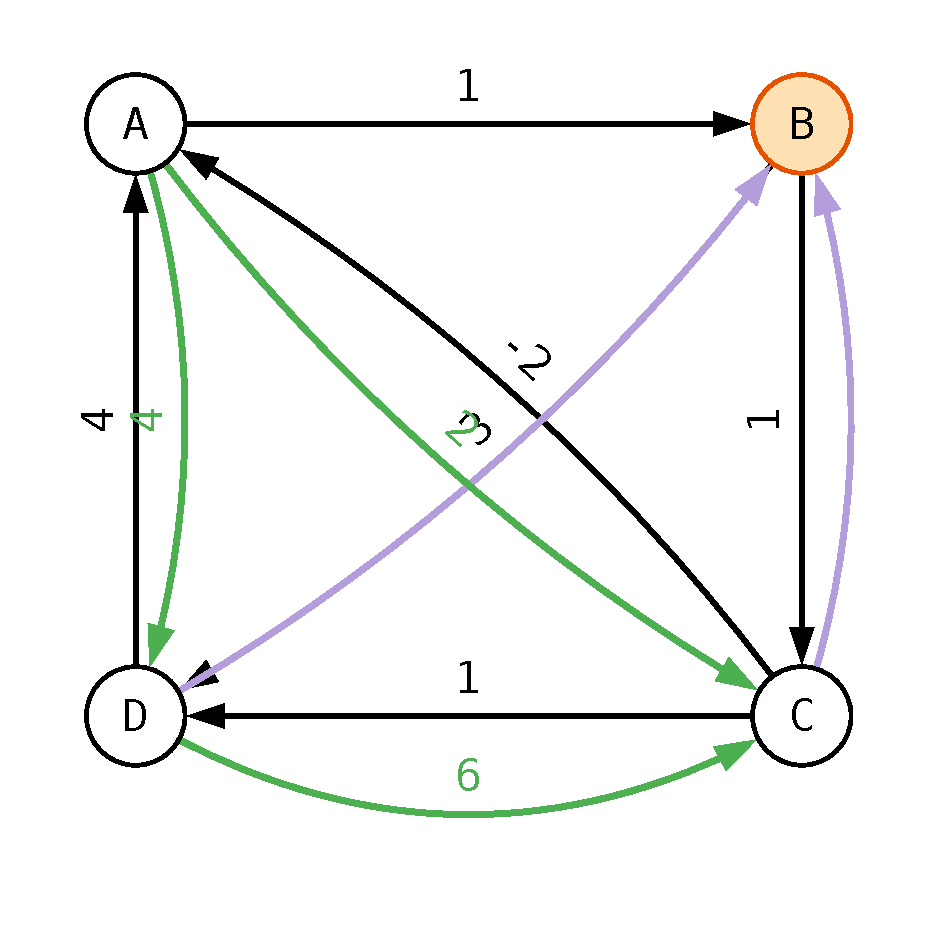
\includegraphics[width=0.30\textwidth]{python/lec14/floyd/floyd-2.pdf}\\[2pt]{\scriptsize Шаг 2. Через $B$: $AC{=}2$, $AD{=}4$, $DC{=}6$}} \\
\end{tabular}\end{center}
\begin{center}\begin{tabular}{cc}
\shortstack{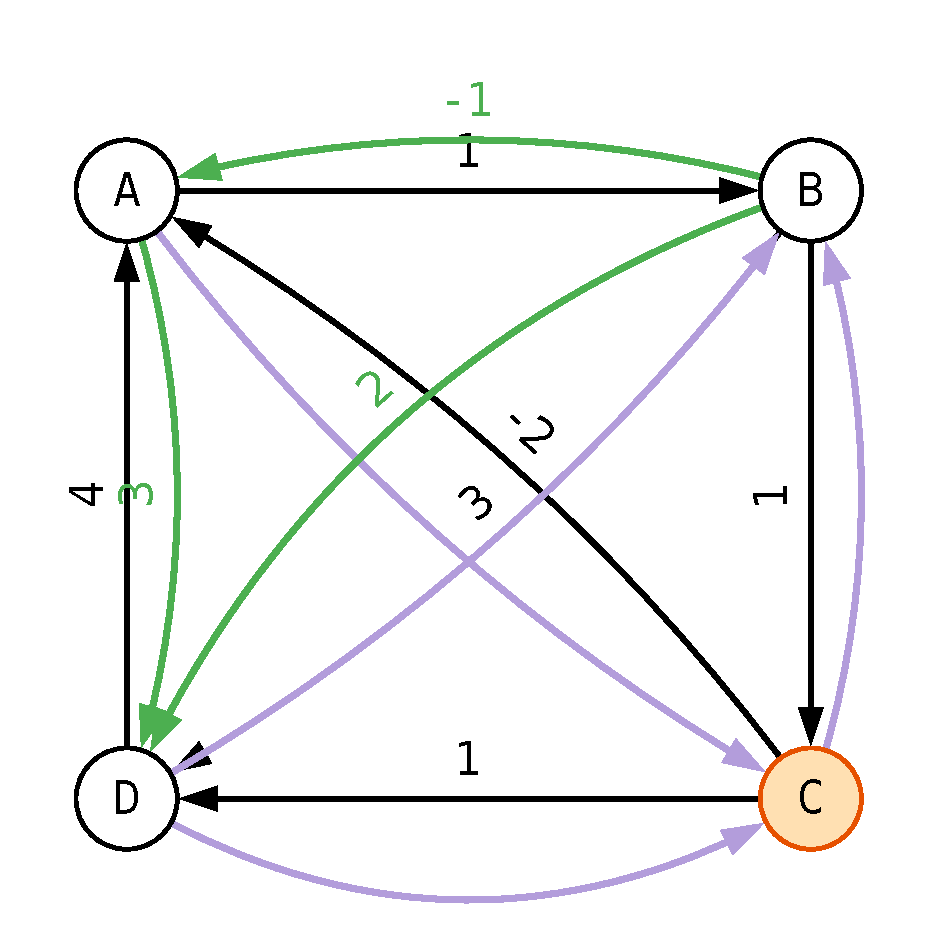
\includegraphics[width=0.30\textwidth]{python/lec14/floyd/floyd-3.pdf}\\[2pt]{\scriptsize Шаг 3. Через $C$: $AD{=}3$, $BA{=}{-}1$, $BD{=}2$}} &
\shortstack{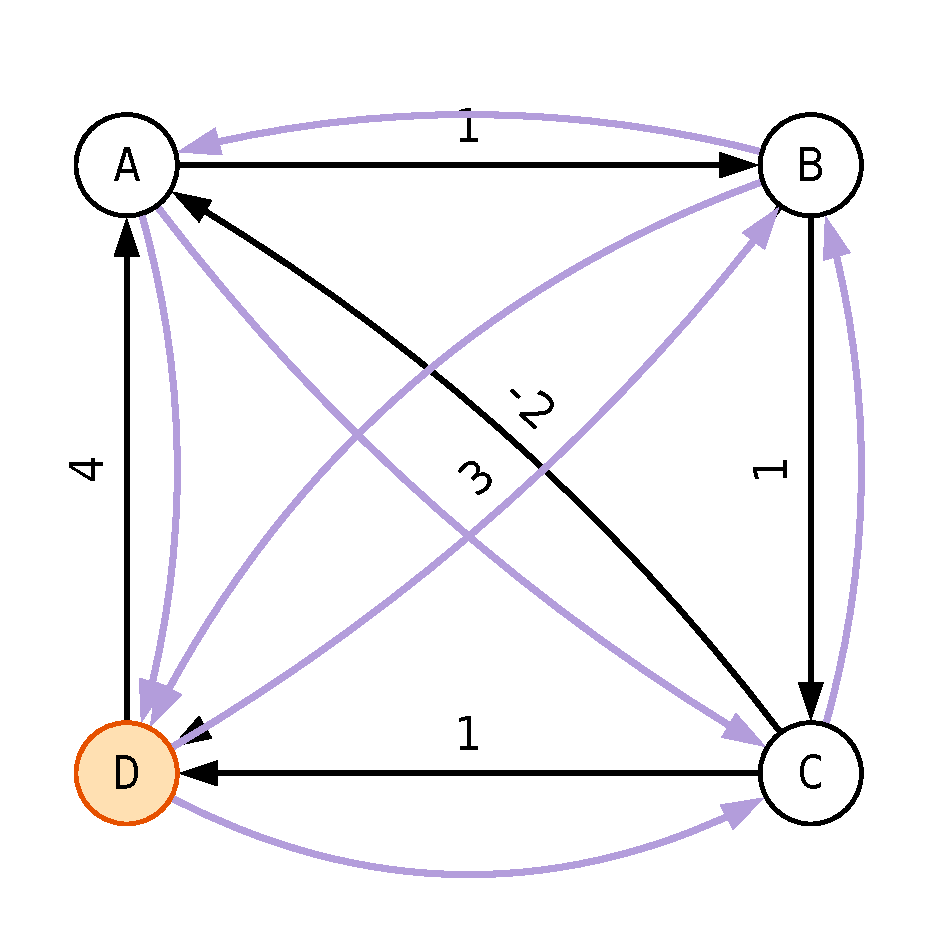
\includegraphics[width=0.30\textwidth]{python/lec14/floyd/floyd-4.pdf}\\[2pt]{\scriptsize Шаг 4. Через $D$ обновлений нет --- итог}} \\
\end{tabular}\end{center}

\textbf{Восстановление путей:}

$A \to D$: $P_{AD} = B$. $A \xrightarrow{1} B$, $P_{BD} = C$, $B \xrightarrow{1} C$, $P_{CD}$ пуст, $C \xrightarrow{1} D$. Итого: $A \xrightarrow{1} B \xrightarrow{1} C \xrightarrow{1} D$, длина $= 3$.

$C \to B$: $P_{CB} = A$. $C \xrightarrow{-2} A$, $P_{AB}$ пуст, $A \xrightarrow{1} B$. Итого: $C \xrightarrow{-2} A \xrightarrow{1} B$, длина $= -1$.

\medskip
\textbf{Циклы отрицательного суммарного веса} $\Leftrightarrow$ отрицательные значения на главной диагонали.

\textit{Почему:} диагональный элемент $\mu(v, v)$ --- длина кратчайшего
замкнутого маршрута через $v$; он станет отрицательным в точности тогда,
когда через $v$ проходит цикл отрицательного веса. Здесь диагональ
нулевая: например, цикл $A \to B \to C \to A$ весит $1 + 1 - 2 = 0$,
отрицательных циклов нет.

\end{algo}

% ===========================================================
%  Алгоритм Джонсона
% ===========================================================

\begin{algo}{Алгоритм Джонсона}{johnson}

Преобразование графа к виду с неотрицательными весами рёбер с сохранением набора кратчайших путей.

$G(V, E)$~--- слабо связный, $\sigma\colon E \to \mathbb{R}$.

\textbf{Идея.} Дейкстра быстрее Флойда ($|V|$ запусков Дейкстры дешевле
при разреженных графах), но не работает с отрицательными рёбрами.
Джонсон <<выпрямляет>> веса потенциалами так, что все веса становятся
неотрицательными, а кратчайшие пути не меняются.

\textbf{Шаг 1. Джонсоновский потенциал.}

Добавляем фиктивную вершину $S$: $\forall\, u \in V\colon e_u = Su$, $\sigma(e_u) = 0$.

\grfig[0.45]{figures/p33-jonson-example-1.pdf}{Алг. Джонсона: тот же граф + фиктивная $S$ (синие дуги веса 0)}

Запускаем \textbf{алгоритм Форда--Беллмана} от $S$ (Дейкстру пока
нельзя --- веса ещё отрицательные); $h(u) :=$ найденное расстояние от
$S$ до $u$.

Результат Форда--Беллмана (потенциалы):
\[
  h(A) = -2, \quad h(B) = -1, \quad h(C) = h(D) = 0.
\]
(Проверка: до $C$ и $D$ дешевле всего прямые нулевые дуги из $S$, т.\,е.
$h(C) = h(D) = 0$; до $A$ выгоден путь $S \to C \to A$ весом
$0 + (-2) = -2$; до $B$ --- путь $S \to C \to A \to B$ весом
$0 - 2 + 1 = -1$.)

\textbf{Шаг 2. Пересчёт весов.}

Новая весовая функция:
\[
  \tilde{\sigma}(\overline{uv}) = \sigma(\overline{uv}) + h(u) - h(v) \geq 0.
\]

\textit{Почему $\tilde\sigma \ge 0$:} $h$ --- корректные расстояния от
$S$, поэтому для любого ребра $uv$ выполнено неравенство треугольника
$h(v) \le h(u) + \sigma(uv)$, что и означает
$\sigma(uv) + h(u) - h(v) \ge 0$.

\begin{center}
\begin{tabular}{c|c|c|l}
Ребро & $\sigma$ & $\tilde{\sigma}$ & Вычисление \\
\hline
$AB$ & 1 & 0 & $1 + (-2) - (-1) = 0$ \\
$BC$ & 1 & 0 & $1 + (-1) - 0 = 0$ \\
$BD$ & 3 & 2 & $3 + (-1) - 0 = 2$ \\
$CA$ & $-2$ & 0 & $-2 + 0 - (-2) = 0$ \\
$CD$ & 1 & 1 & $1 + 0 - 0 = 1$ \\
$DA$ & 4 & 6 & $4 + 0 - (-2) = 6$ \\
\end{tabular}
\end{center}

\grfig[0.42]{figures/p33-jonson-2.pdf}{Перевешенный граф: все $\tilde\sigma \ge 0$}

Все $\tilde{\sigma} \geq 0$~--- можно применять Дейкстру!

\textbf{Шаг 3. Дейкстра от каждой вершины} с весами $\tilde{\sigma}$.

Матрица расстояний в весах $\tilde\sigma$:
\begin{center}
\begin{tabular}{c|cccc}
$\mathrm{dist}_{\tilde\sigma}$ & $A$ & $B$ & $C$ & $D$ \\
\hline
$A$  & 0 & 0 & 0 & 1 \\
$B$  & 0 & 0 & 0 & 1 \\
$C$  & 0 & 0 & 0 & 1 \\
$D$  & 6 & 6 & 6 & 0 \\
\end{tabular}
\end{center}

(Например, из $D$: единственный выход --- дуга $DA$ веса $6$, дальше
всё бесплатно по нулевым дугам $A \to B \to C$; поэтому вся строка $D$
равна $6$.)

\textbf{Шаг 4. Обратный пересчёт.}

Для получения истинных расстояний:
\[
  \mathrm{dist}_\sigma(u,v) = \mathrm{dist}_{\tilde\sigma}(u,v) - h(u) + h(v).
\]

\textit{Почему пути не изменились:} для любого пути
$u = x_0 \to x_1 \to \ldots \to x_k = v$ его новая длина равна
\[
  \sum_i \tilde\sigma(x_i x_{i+1})
  = \sum_i \sigma(x_i x_{i+1}) + h(u) - h(v)
\]
--- телескопическая сумма: все промежуточные потенциалы сокращаются.
Все пути из $u$ в $v$ сдвинулись на \emph{одну и ту же} константу
$h(u) - h(v)$, поэтому порядок путей по длине (и сами кратчайшие пути)
сохранился, а формула пересчёта очевидна.

Итоговая матрица истинных расстояний
($\mathrm{dist}_\sigma = \mathrm{dist}_{\tilde\sigma} - h(u) + h(v)$):
\begin{center}
\begin{tabular}{c|cccc}
$\mathrm{dist}_{\sigma}$ & $A$ & $B$ & $C$ & $D$ \\
\hline
$A$  & 0    & 1    & 2 & 3 \\
$B$  & $-1$ & 0    & 1 & 2 \\
$C$  & $-2$ & $-1$ & 0 & 1 \\
$D$  & 4    & 5    & 6 & 0 \\
\end{tabular}
\end{center}

Например, $\mathrm{dist}_\sigma(D, A) = 6 - h(D) + h(A) = 6 - 0 - 2 = 4$;
$\mathrm{dist}_\sigma(B, A) = 0 - (-1) + (-2) = -1$. Матрица совпала с
результатом алгоритма Флойда выше --- проверка пройдена. $\checkmark$

\textbf{Свойства:}
\begin{enumerate}
  \item Набор кратчайших путей для $G$ в терминах $\sigma$ и $\tilde{\sigma}$ совпадает (пути не меняются, только длины) --- телескопическая сумма выше.
  \item $\forall\, e \in E\colon \tilde{\sigma}(e) \geq 0$ (неравенство треугольника для корректных потенциалов).
  \item Если $\tilde{\sigma}(e) < 0$ для какого-то ребра~--- значит, потенциалы найдены неправильно.
\end{enumerate}

\end{algo}

% ============================================================
\begin{task}{Кратчайшие пути между всеми парами: алгоритм Флойда}{floyd-task}
\textbf{Условие.} Дан ориентированный взвешенный граф на вершинах $A,B,C,D$ с
дугами
\[
  A\!\to\!B=3,\ A\!\to\!C=8,\ B\!\to\!C=2,\ B\!\to\!D=5,\ C\!\to\!D=1,\ D\!\to\!A=2.
\]
Найдите кратчайшие расстояния между всеми парами вершин алгоритмом Флойда.

\begin{center}
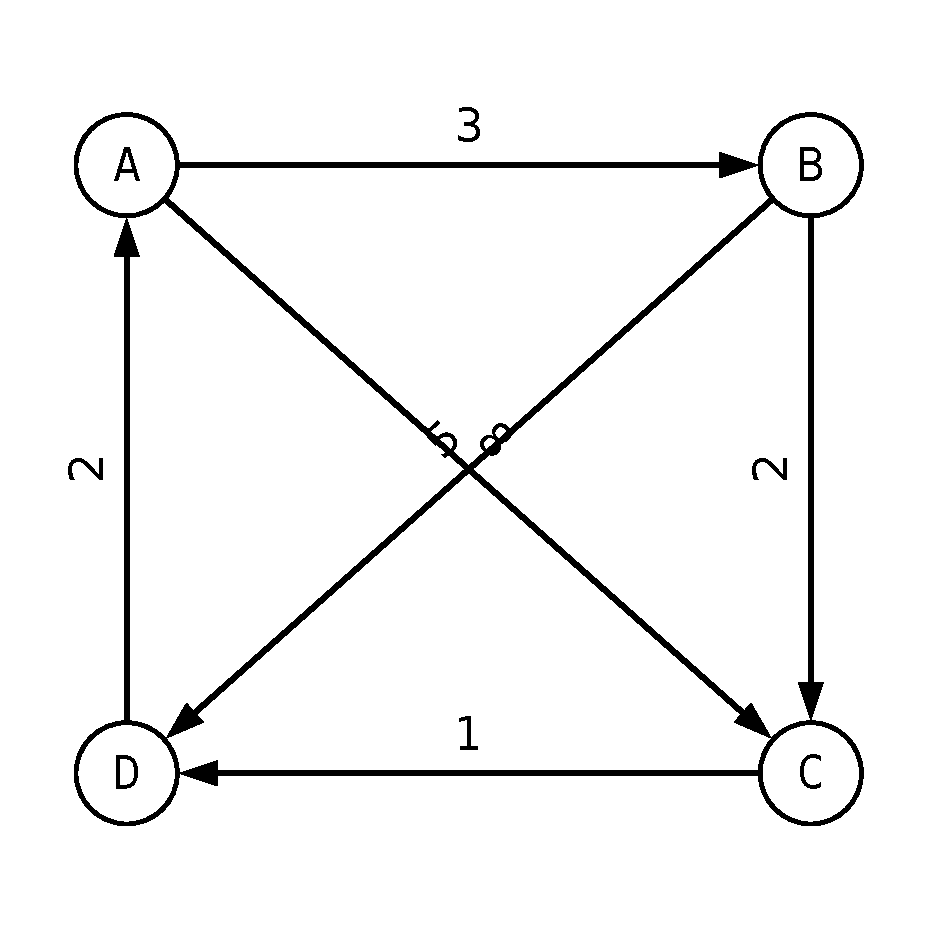
\includegraphics[width=0.42\textwidth]{figures/task-floyd-1.pdf}
\end{center}

\smallskip
\textbf{Решение.} Флойд последовательно разрешает в качестве промежуточных
вершины $A,B,C,D$. На шаге $k$ обновляем
$d[i][j]\leftarrow\min\bigl(d[i][j],\,d[i][k]+d[k][j]\bigr)$.

Начальная матрица $D^{(0)}$ (на диагонали $0$, отсутствующие дуги --- $\infty$):
\begin{center}
\renewcommand{\arraystretch}{1.25}
\begin{tabular}{|c||c|c|c|c|}
\hline
$D^{(0)}$ & \textbf{A} & \textbf{B} & \textbf{C} & \textbf{D} \\ \hline\hline
\textbf{A} & 0 & 3 & 8 & $\infty$ \\ \hline
\textbf{B} & $\infty$ & 0 & 2 & 5 \\ \hline
\textbf{C} & $\infty$ & $\infty$ & 0 & 1 \\ \hline
\textbf{D} & 2 & $\infty$ & $\infty$ & 0 \\ \hline
\end{tabular}
\end{center}

\noindent\textbf{Через $A$:} обновляются пути из $D$ ($D\!\to\!A=2$):
$D\!\to\!B=2+3=5$, $D\!\to\!C=2+8=10$.

\noindent\textbf{Через $B$:} $A\!\to\!C=\min(8,3+2)=5$, $A\!\to\!D=3+5=8$;
$D\!\to\!C=\min(10,5+2)=7$.

\noindent\textbf{Через $C$:} $A\!\to\!D=\min(8,5+1)=6$, $B\!\to\!D=\min(5,2+1)=3$.

\noindent\textbf{Через $D$:} замыкаются обратные пути:
$B\!\to\!A=3+2=5$, $C\!\to\!A=1+2=3$, $C\!\to\!B=1+2+3=6$ и т.\,д.

Итоговая матрица кратчайших расстояний $D^{(4)}$:
\begin{center}
\renewcommand{\arraystretch}{1.25}
\begin{tabular}{|c||c|c|c|c|}
\hline
$D^{(4)}$ & \textbf{A} & \textbf{B} & \textbf{C} & \textbf{D} \\ \hline\hline
\textbf{A} & 0 & 3 & 5 & 6 \\ \hline
\textbf{B} & 5 & 0 & 2 & 3 \\ \hline
\textbf{C} & 3 & 6 & 0 & 1 \\ \hline
\textbf{D} & 2 & 5 & 7 & 0 \\ \hline
\end{tabular}
\end{center}

Проверка: $B\!\to\!A$ идёт по маршруту $B\!\to\!C\!\to\!D\!\to\!A=2+1+2=5$;
$C\!\to\!B=C\!\to\!D\!\to\!A\!\to\!B=1+2+3=6$ --- совпадает с таблицей.

\textbf{Ответ.} Матрица кратчайших расстояний $D^{(4)}$ приведена выше.
\end{task}
